\documentclass{article}
\usepackage[UTF8]{ctex}
\usepackage{amsmath,mathtools,geometry,pgfplots,float,mathrsfs,caption,enumerate}
\pgfplotsset{compat=1.15}
\usetikzlibrary{arrows}
\geometry{scale=0.7}

\title{每日一题(16.1)}
\author{\kaishu 李政毅}
\date{2022年5月10日}

\begin{document}
\maketitle
\begin{enumerate}
	\renewcommand{\labelenumi}{\textbf{\theenumi. }}
	\item 判断说理, 正确的说明理由, 错误的举出反例.\par
	已知$\triangle ABC$的三边长分别为$a$, $b$, $c$.
	\begin{enumerate}[(1) ]
		\item 以$\dfrac{1}{a}$, $\dfrac{1}{b}$, $\dfrac{1}{c}$为三边的三角形一定存在;
		\item 以$|a-b|+1$, $|b-c|+1$, $|c-a|+1$为三边的三角形一定存在.
	\end{enumerate}
	
	\item 如图, 把一个三角形纸片$ABC$的三个顶点向内折叠之后, 求\[\angle\alpha_1+\angle\alpha_2+\angle\beta_1+\angle\beta_2+\angle\gamma_1+\angle\gamma_2.\]
	\begin{figure}[htbp]
		\flushright
		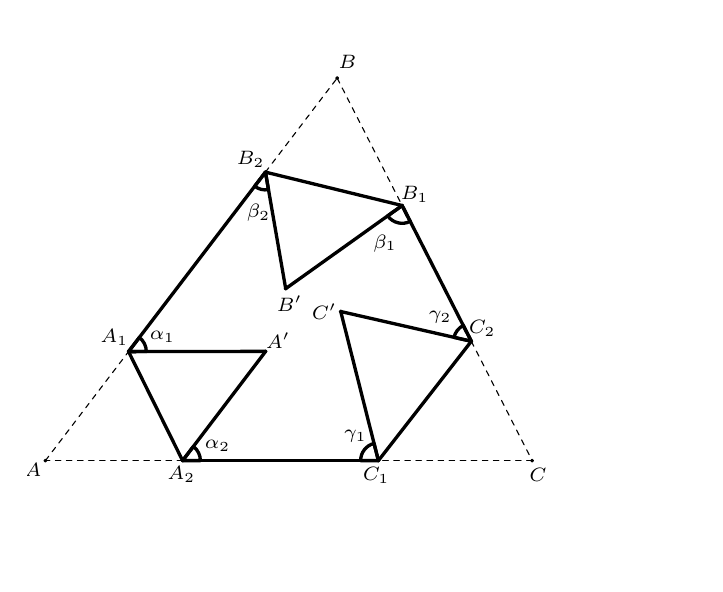
\begin{tikzpicture}[line cap=round,line join=round,>=triangle 45,x=1.0cm,y=1.0cm]
			\clip(-0.2253440260140864,-1.3150277809891584) rectangle (8.242504223943547,5.498213294834198);
			\draw [shift={(2.79441672731757,3.6637436986301997)},line width=1.2pt] (0,0) -- (-127.33355107820586:0.22560400913322398) arc (-127.33355107820586:-80.14794815820449:0.22560400913322398) -- cycle;
			\draw [shift={(4.530444146372828,3.2392375434929965)},line width=1.2pt] (0,0) -- (-144.48969367721884:0.22560400913322398) arc (-144.48969367721884:-62.99180555919153:0.22560400913322398) -- cycle;
			\draw [shift={(5.409070192199978,1.515446351879068)},line width=1.2pt] (0,0) -- (117.00819444080847:0.22560400913322398) arc (117.00819444080847:167.16461847950927:0.22560400913322398) -- cycle;
			\draw [shift={(4.2287498521774864,0.)},line width=1.2pt] (0,0) -- (104.17281292031771:0.22560400913322398) arc (104.17281292031771:180.:0.22560400913322398) -- cycle;
			\draw [shift={(1.742514247281429,0.)},line width=1.2pt] (0,0) -- (0.:0.22560400913322398) arc (0.:52.764644072060634:0.22560400913322398) -- cycle;
			\draw [shift={(1.0558588948814451,1.3843305241297743)},line width=1.2pt] (0,0) -- (0.09819515026647681:0.22560400913322398) arc (0.09819515026647681:52.666448921794164:0.22560400913322398) -- cycle;
			\draw [line width=1.2pt] (1.0558588948814451,1.3843305241297743)-- (1.742514247281429,0.);
			\draw [line width=1.2pt] (2.79441672731757,3.6637436986301997)-- (4.530444146372828,3.2392375434929965);
			\draw [line width=1.2pt] (5.409070192199978,1.515446351879068)-- (4.2287498521774864,0.);
			\draw [line width=0.4pt,dash pattern=on 2pt off 2pt] (2.79441672731757,3.6637436986301997)-- (3.705331830094106,4.858039250599726);
			\draw [line width=0.4pt,dash pattern=on 2pt off 2pt] (3.705331830094106,4.858039250599726)-- (4.530444146372828,3.2392375434929965);
			\draw [line width=1.2pt] (4.530444146372828,3.2392375434929965)-- (5.409070192199978,1.515446351879068);
			\draw [line width=0.4pt,dash pattern=on 2pt off 2pt] (5.409070192199978,1.515446351879068)-- (6.1815017037962505,0.);
			\draw [line width=0.4pt,dash pattern=on 2pt off 2pt] (6.1815017037962505,0.)-- (4.2287498521774864,0.);
			\draw [line width=1.2pt] (4.2287498521774864,0.)-- (1.742514247281429,0.);
			\draw [line width=0.4pt,dash pattern=on 2pt off 2pt] (1.742514247281429,0.)-- (0.,0.);
			\draw [line width=0.4pt,dash pattern=on 2pt off 2pt] (0.,0.)-- (1.0558588948814451,1.3843305241297743);
			\draw [line width=1.2pt] (1.0558588948814451,1.3843305241297743)-- (2.79441672731757,3.6637436986301997);
			\draw [line width=1.2pt] (3.0514218434680864,2.183859730140428)-- (2.79441672731757,3.6637436986301997);
			\draw [line width=1.2pt] (3.0514218434680864,2.183859730140428)-- (4.530444146372828,3.2392375434929965);
			\draw [line width=1.2pt] (3.750623731158658,1.893313287969004)-- (5.409070192199978,1.515446351879068);
			\draw [line width=1.2pt] (3.750623731158658,1.893313287969004)-- (4.2287498521774864,0.);
			\draw [line width=1.2pt] (1.742514247281429,0.)-- (2.7968930997874786,1.3873143614072445);
			\draw [line width=1.2pt] (1.0558588948814451,1.3843305241297743)-- (2.7968930997874786,1.3873143614072445);
			\begin{scriptsize}
				\draw [fill=black] (0.,0.) circle (0.5pt);
				\draw[color=black] (-0.15748504945015954,-0.11556646576418493) node {$A$};
				\draw [fill=black] (3.705331830094106,4.858039250599726) circle (0.5pt);
				\draw[color=black] (3.835705912207905,5.065805610662187) node {$B$};
				\draw [fill=black] (6.1815017037962505,0.) circle (0.5pt);
				\draw[color=black] (6.257188943571175,-0.17572753486637793) node {$C$};
				\draw [fill=black] (1.0558588948814451,1.3843305241297743) circle (0.5pt);
				\draw[color=black] (0.8765333257437837,1.5651834022783317) node {$A_1$};
				\draw [fill=black] (1.742514247281429,0.) circle (0.5pt);
				\draw[color=black] (1.7263084268122608,-0.17196746804749083) node {$A_2$};
				\draw [fill=black] (2.79441672731757,3.6637436986301997) circle (0.5pt);
				\draw[color=black] (2.6061640624318345,3.8212234936105687) node {$B_2$};
				\draw [fill=black] (4.530444146372828,3.2392375434929965) circle (0.5pt);
				\draw[color=black] (4.689241080095269,3.377535608981895) node {$B_1$};
				\draw [fill=black] (5.409070192199978,1.515446351879068) circle (0.5pt);
				\draw[color=black] (5.54653631480152,1.6779854068449436) node {$C_2$};
				\draw [fill=black] (4.2287498521774864,0.) circle (0.5pt);
				\draw[color=black] (4.20043239363995,-0.18700773532303908) node {$C_1$};
				\draw [fill=black] (3.0514218434680864,2.183859730140428) circle (0.5pt);
				\draw[color=black] (3.09873281570604,1.9900709528125697) node {$B'$};
				\draw [fill=black] (2.7968930997874786,1.3873143614072445) circle (0.5pt);
				\draw[color=black] (2.9558502765883317,1.523822667270574) node {$A'$};
				\draw [fill=black] (3.750623731158658,1.893313287969004) circle (0.5pt);
				\draw[color=black] (3.542420700334714,1.892309215521506) node {$C'$};
				\draw[color=black] (2.706566735187317,3.1444114662108973) node {$\beta_2$};
				\draw[color=black] (4.31318273702012,2.7608846506844174) node {$\beta_1$};
				\draw[color=black] (5.012606826519557,1.8186296832537155) node {$\gamma_2$};
				\draw[color=black] (3.9372277163178557,0.30932108477005305) node {$\gamma_1$};
				\draw[color=black] (2.185036578716483,0.18899894656566707) node {$\alpha_2$};
				\draw[color=black] (1.4856641504034884,1.572703535916106) node {$\alpha_1$};
			\end{scriptsize}
		\end{tikzpicture}
	\end{figure}
\end{enumerate}
\end{document}